%======================================================================
\chapter{Implementation}
\label{ch: implementation}
%======================================================================

For the implementation of this project we had to start from scratch since this was a new project concept introduced by our advisor Dr. Miah. There have been senior projects in the past that have used XBees to get signal strength but there is very little overlap between these projects to substantiate where our project needed to start from. For this project we had to first build a mobile robot and a remote to use for testing. We then had to build a code base to control the mobile robot that was then implemented with our test algorithms.

%----------------------------------------------------------------------
\section{Robot Assembly}
\label{sec:Robot Assembly}
%----------------------------------------------------------------------

For this project we needed a Remote Target and Smart Robotic Cart that we designed and implemented from off the shelf components.  As mentioned above in section \ref{sec:System Components}, some of our components came from what the school already owned as well as some we had to buy specifically for this project listed in \autoref{tab:Partslablist} and \autoref{tab:Partslist}.

\vspace*{12pt}
\noindent
Since the school already owned the Budget Bot chassis, we decided to build our Smart Robotic Cart with them. The Budget Bot chassis needed to be modified slightly to work with our project. The main change we made was swapping out the motors that came with the Budget Bot for Pololu 27D Metal Gear motors since the original motors have a max speed of 212 RPM or 1.09m/s and the new motors have a max speed of 530 RPM or 2.72m/s when using the wheels with a diameter of 98mm. By switching out the motors we are able to achieve our goal of matching an average person's walking speed of 1.5m/s. The other modifications to the chassis are a hard power switch to directly cut off power to the XBee modules in the reflector and a power indicator LED to let us know when this switch was on.

\vspace*{12pt}
\noindent
As shown in Fig. \ref{fig:FinalizedRobot}, our next step was to attach the BeagleBone Blue microcomputer, XBee reflector array assembly, and breadboard to the top of the robot. We also installed a 2-cell LiPo battery inside the chassis of the mobile cart that delivers power to the BeagleBone Blue directly and the breadboard through the switch.

\begin{figure}[H]
    \centering
    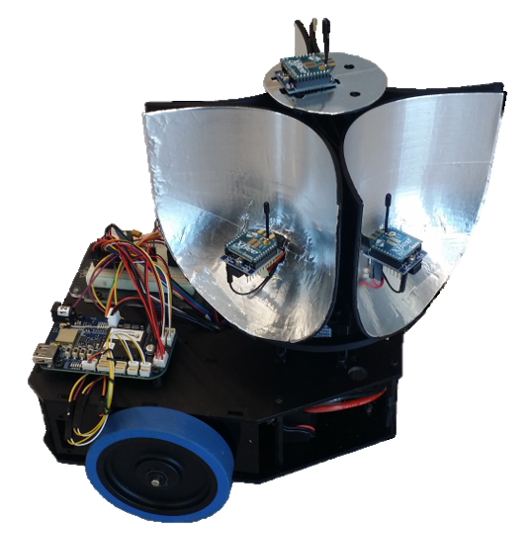
\includegraphics[width=0.5\textwidth]{figs/img/Finalized_robot.png}
    \caption{Overall Prototype of the Robotic Cart}
    \label{fig:FinalizedRobot}
\end{figure}

The power supplied to the breadboard is sent through a regulator circuit to drop it down from the 7.4V of the LiPo to 3.3V of the XBee. This circuit is also used on the remote which consists of a 7.4V LiPo battery and the XBee module with voltage regulator in between. This voltage regulator is built out of a LM117 regulator and a 10uF ceramic capacitor between the input and output pins of the regulator as shown in Fig. \ref{fig:PowerConverter}.

\begin{figure}[H]
    \centering
    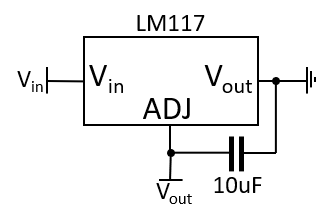
\includegraphics[width=0.5\textwidth]{figs/img/PowerConverter.png}
    \caption{Final Version of the Robotic Cart}
    \label{fig:PowerConverter}
\end{figure}

\vspace*{12pt}
\noindent
The reflector array assembly from \autoref{sec:customReflector} was mounted on a stepper motor that was then attached to the robot chassis using a 3D printed bracket. This bracket was then attached to the chassis using bolts. Another feature of this bracket is that it had a stop block built into the top of it to automatically zero the reflector array when the robot starts up.

\vspace*{12pt}
\noindent
The Xbee modules from the reflector array posed a bit of a problem when it came to connecting them to the BeagleBone Blue. This problem comes from that the BeagleBone Blue has five UART ports if we are using the one found in the USB and the UART-GPS along with the three normal UART ports.\todo[inline]{This sentence needs to be revised. -Kalli} This does not work since UART port zero is tied to the council used to communicate with it from a computer. Since this port is reserved for this function that reduces the number of usable ports down to four and we need to have five XBees in these ports. Our solution to this was to use two of the GPIO pins, two of the UART ports, and a two-way multiplexer. With this setup we can directly connect one of the UARTs to the top XBee and then rout the other four side XBee modules through the MUX so only one UART port is needed for them.


%----------------------------------------------------------------------
\section{Code Base}
\label{sec:Code Base}
%----------------------------------------------------------------------

For the project we needed some base functionality to use with the main follower program so it can interact with the other components in the system. The BeagleBone Blue already has a set of ports on it that we can access and control using the Robot Control Library from Strawson Design ~\cite{Robot_Control_Library}.

\vspace*{12pt}
\noindent
For the project we also built some custom libraries on top of the Robot Control Library to handle XBee Frames, AT Commands, and the stepper motor. The XBee Frames library takes a given block of data containing our message and then packages it into a XBee Frame to send over UART to the XBee module we want to interact with. The XBee communications library also handles received messages from the XBee module and validates the received frames integrity and extracts the message data from it. On top of the XBee communications library we also have a library that generates AT Commands to package in the XBee Frames. The AT Command library also handles extracting response data from the AT Response Command structure and validates it.

\begin{figure}[H]
  \centering
  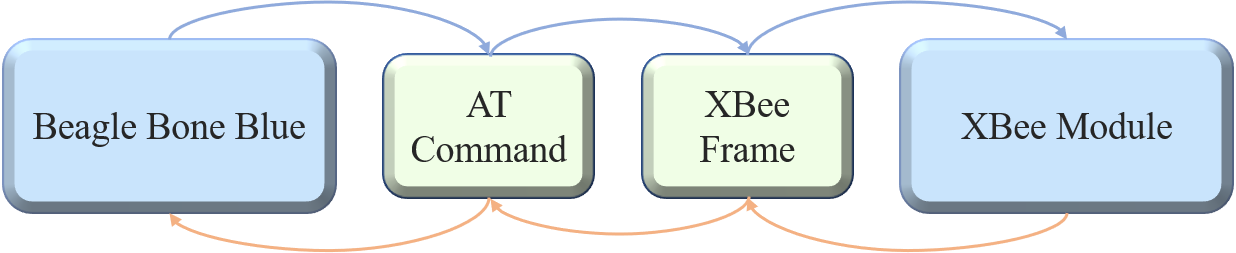
\includegraphics[width=\textwidth]{figs/img/Command Process Diagram.png}
  \caption{Process for XBee Communication over UART}
  \label{fig:CommandProcessDiagram}
\end{figure}

\vspace*{12pt}
\noindent
The final custom library is the stepper motor control library. This library had to be written ourselves since instead of using a dedicated stepper motor controller for our project we were using two of the regular DC motor control ports that are build into the BeagleBone Blue. The library handled translating how many steps to turn into proper cycling of the DC motor ports to get the stepper motor to move the desired distance. \todo[inline]{This sentence needs to be revised since it makes no sense. -Kalli} The library also helped to keep track of basic information related to the stepper motor such as what its current angle should be.

%----------------------------------------------------------------------
\section{Experimental Results}
\label{sec:Experimental Results}
%----------------------------------------------------------------------

In this project after we had the Robotic Cart, Remote Target, and a code base to handle the specifics we started testing different variants of our algorithm explained in \autoref{sec:locAndNavAlgos}. There were two main types of variants we put together, one type the stepper motor is locked preventing the reflector from turning and in the other we use the stepper motor to sweep through a set of angles.

\subsection{Rotating Reflector Tests}

The first type of test we ran was where the robot would zero out the arrays rotation with the stepper motor then move in nine degree increments taking measurements as it went. A sweep ends when the motor has turned 81 degrees since at that point, with the four sides of the reflector, a full 360 degrees has bean scanned.

\vspace*{12pt}
\noindent
This method offers us a sufficiently dense set of data to base our angle predictions off of but at the cost of having to wait until a entire sweep of the reflectors is completed. With this data we first put together a simple test that would continuously be sweeping and moving at the same time. Though this version did successfully follow the remote it had some errors in the robot's navigation trajectory. For example, the robot would correctly turn towards the remote, however, if it picked up a stronger signal from the XBee reverberations, it would drive off in a different direction. The robot would eventually find its way back into alignment and resume moving towards the remote.

\vspace*{12pt}
\noindent
\todo[inline]{This section needs to be fixed. You have some wording issues that makes it hard for me to understand what you are saying. -Kalli}
The next version that used a rotating reflector as well as the final version works mostly the same as the first version but with some improvements to its navigation.  The first big fix is that we determined that the result of the oscillation we were seeing in the first test was a result of turning while also rotating the reflector which would add additional rotation to the measurements in global scope. Due to how our robot is designed we can only rotate the reflector array 90 degrees but to properly fix this rotation issue we would need to rotate the reflector more or less during a sweep to compensate for the robots rotation. Our compromise was simply to allow the robot to always move forward but to alternate between rotating the reflector and getting a measurement and then rotating the robot based on that measurement. In this version we also added some additional windowed filters to average out the angle measurements which did help to reduce the effects of random angles from noise in the system. We also applied offsets to each of the directional receivers revived signal strengths based off of data that we had collected while testing it when we noticed that each side had a different minimum that it would cap out at.

\subsection{Locked Reflector Tests}

The locked reflector tests were ran in between our first algorithm and our final algorithm which ultimately used a sweeping function to capture the XBee signals. These algorithms were an attempt to reduce the time needed to get a set of measurements from the reflector by zeroing its rotation and then keeping it locked in the zeroed position. Since the data from this is relatively sparse we tried three different ways to fill in the gaps in the data from only the four cardinal directions. The first of these three methods was to try and select a strongest direction that the signal was coming from and then which of its two neighbor directions had the next strongest signal. With these two strengths the algorithm would then try to interpolate between these two angles based on the difference of the strengths between them. This method could work but due to the time constraints of our project, we did not have enough time to implement and test this method.

\vspace*{12pt}
\noindent
The other two methods that we tried with the locked reflector were both different variants on machine learning algorithms based on a small pool of data we had collected. The first algorithm tested was K Nearest Neighbors then followed up by a Neural Network for our final fixed rotation test. Both of these algorithms failed to produce any meaningful results due to the fact that we had a very small pool of data to work off of compared to the large amounts of data needed to perform machine learning algorithms. These algorithms, with the small data pool size, did not perform well with the noise in the signals.

\subsection{System noise}

In both our fixed and sweeping experiments a underlying issue is the amount of noise our system produces. The first type of noise that occurs is noise from the Multipath Effect where the signals bounce off of obstacles around it adding constructing and destructive interference randomly based off of the robots surroundings. The second noise was from internal noise in the XBees which was worse that we had expected. We managed to isolate the XBee internal noise by using an anechoic chamber where we did see all the signals strengths become stronger but the base noise from the XBees persisted. The noise coming from the XBees tends to be about 2 to 6 dBm on average. The change from facing towards the remote then away from the remote is about 13 to 15 dBm. These ranges result in the occasional measurement that flip flops which reflector is actually facing the remote. The noise can be seen in our test measurements we collected where we, at set rotations, record a burst of 300 measurements as seen in Fig. \ref{fig:SensorDataGraphs}

\begin{figure}[H]
    \centering
    \begin{subfigure}{0.50\textwidth}
        \centering
        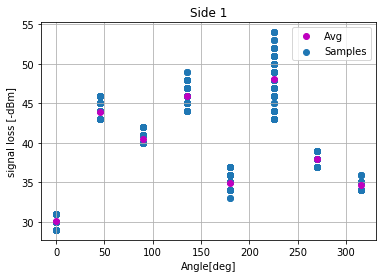
\includegraphics[width=0.95\textwidth]{figs/img/Side1_Data.png}
        \label{fig:Side1Dat}
    \end{subfigure}%
    \begin{subfigure}{0.50\textwidth}
        \centering
        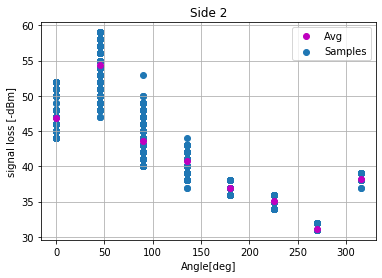
\includegraphics[width=0.95\textwidth]{figs/img/Side2_Data.png}
        \label{fig:Side2Dat}
    \end{subfigure}
        \begin{subfigure}{0.50\textwidth}
        \centering
        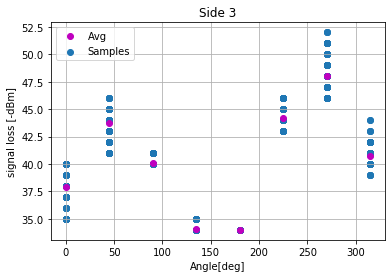
\includegraphics[width=0.95\textwidth]{figs/img/Side3_Data.png}
        \label{fig:Side3Dat}
    \end{subfigure}%
    \begin{subfigure}{0.50\textwidth}
        \centering
        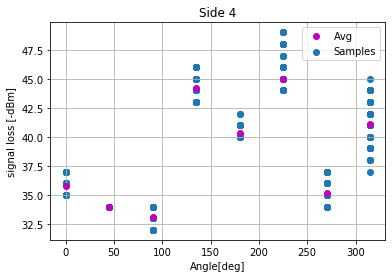
\includegraphics[width=0.95\textwidth]{figs/img/Side4_Data.png}
        \label{fig:Side4Dat}
    \end{subfigure}
    \caption{Navigation Algorithm Details}
    \label{fig:SensorDataGraphs}
\end{figure}

\subsection{Distance}

\todo[inline]{Was going back over this and realized I should add this section in will do later don't have time at this exact moment. -Darrah}



\section{Simulation using Robot Simulator}

Before constructing the physical robot prototype, a simulation was performed using a commercial robot simulator CoppeliaSim. However, since RF signal behavior depends highly on the environment, the system could not be fully simulated. This section explains the steps taken to simulate the proposed robotic cart.

\vspace*{12pt}
\noindent
First, a model of the Budget Bot chassis was created in CoppeliaSim. The model is shown in Fig. \ref{fig:budgetBotModel}. The model was designed with the same dimensions as the physical chassis to accurately simulate the robot kinematics. Details on modeling a robot chassis in CoppeliaSim can be found in \autoref{ch: coppSimModeling}. Although \autoref{ch: coppSimModeling} explains the modeling of a robot chassis that is different than the Budget Bot chassis, the concepts are the same for modeling any robot chassis.

\begin{figure}
    \centering
    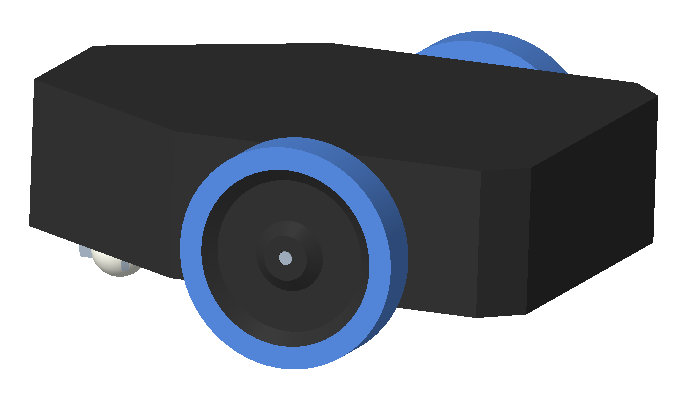
\includegraphics[width=0.6\textwidth]{figs/img/budgetBotModel.png}
    \caption{Model of Budget Bot Chassis}
    \label{fig:budgetBotModel}
\end{figure}

\vspace*{12pt}
\noindent
MATLAB code was written to control the simulation. The actual distance between the robot and the remote was measured, then random noise was added with a mean of 0 and a standard deviation of 0.07. This noisy measurement was then used in the navigation algorithm to determine how to drive the robot (see \autoref{subsec:navAlgo}). An image of the simulation is shown in Fig. \ref{fig:coppSimExample}, where the blue sphere represents the remote, and the green dot represents the target point.
\begin{figure}
    \centering
    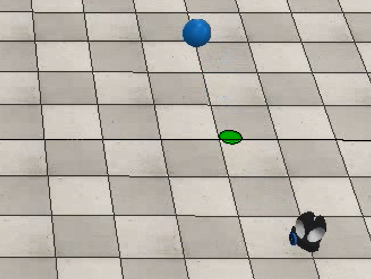
\includegraphics[width=0.5\textwidth]{figs/img/coppSimExample.png}
    \caption{CoppeliaSim Simulation}
    \label{fig:coppSimExample}
\end{figure}


%%% Local Variables:
%%% mode: latex
%%% TeX-master: "../finalReport"
%%% End:
